\chapter{\IfLanguageName{dutch}{Stand van zaken}{State of the art}}%
\label{ch:stand-van-zaken}

% Tip: Begin elk hoofdstuk met een paragraaf inleiding die beschrijft hoe
% dit hoofdstuk past binnen het geheel van de bachelorproef. Geef in het
% bijzonder aan wat de link is met het vorige en volgende hoofdstuk.

% Pas na deze inleidende paragraaf komt de eerste sectie hoofding.

%Dit hoofdstuk bevat je literatuurstudie. De inhoud gaat verder op de inleiding, maar zal het onderwerp van de bachelorproef *diepgaand* uitspitten. De bedoeling is dat de lezer na lezing van dit hoofdstuk helemaal op de hoogte is van de huidige stand van zaken (state-of-the-art) in het onderzoeksdomein. Iemand die niet vertrouwd is met het onderwerp, weet nu voldoende om de rest van het verhaal te kunnen volgen, zonder dat die er nog andere informatie moet over opzoeken \autocite{Pollefliet2011}.

%Je verwijst bij elke bewering die je doet, vakterm die je introduceert, enz.\ naar je bronnen. In \LaTeX{} kan dat met het commando \texttt{$\backslash${textcite\{\}}} of \texttt{$\backslash${autocite\{\}}}. Als argument van het commando geef je de ``sleutel'' van een ``record'' in een bibliografische databank in het Bib\LaTeX{}-formaat (een tekstbestand). Als je expliciet naar de auteur verwijst in de zin, gebruik je \texttt{$\backslash${}textcite\{\}}.
%Soms wil je de auteur niet expliciet vernoemen, dan gebruik je \texttt{$\backslash${}autocite\{\}}. In de volgende paragraaf een voorbeeld van elk.

%\textcite{Knuth1998} schreef een van de standaardwerken over sorteer- en zoekalgoritmen. Experten zijn het erover eens dat cloud computing een interessante opportuniteit vormen, zowel voor gebruikers als voor dienstverleners op vlak van informatietechnologie~\autocite{Creeger2009}.

%\lipsum[7-20]

Het doel van dit onderzoek is om de  installatie van de software die nodig is voor het vak Big Data Processing aan HoGent zoveel mogelijk te automatiseren.
Meer concreet worden tijdens deze oefeningen de applicaties Hadoop, Spark en Kafka gebruikt. Momenteel wordt deze software geïnstalleerd tijdens de les. Lestijd die beter kan besteed worden aan bijvoorbeeld het gebruik van de applicaties.
\newline
\newline
Een extra doelstelling is om deze applicaties ook tijdens de examens te kunnen gebruiken op een centrale installatie van HoGENT, met inachtname van veiligheid en stabiliteit.
\newline
\newline
Typisch is dat er telkens 2 van deze applicaties nodig zijn, bijvoorbeeld Hadoop in combinatie met Spark of Spark in combinatie met Kafka. Meer hierover verder in dit hoofdstuk.
\newline
\newline
Gezien het doel van deze studie is te komen tot een installatie, in de eerste instantie ter ondersteuning van de oefeningen, zal het onderzoek zich vooral richten op de functionaliteiten die tijdens de les gebruikt worden. Daarnaast zijn ook de aspecten voor de installatie van belang. We stippen aan dat we hierbij niet ingaan op de volledige werking van de verschillende software.
\newline
\newline

\section{Containertechnologie}
Container technology is a lightweight, executable unit of software that packs up application code and dependencies such as binary code, libraries, and configuration files for easy deployment across different computing environments \autocite{Solarwinds2023}.

\subsubsection{Container}
Containers are an abstraction at the app layer that packages code and dependencies together. Multiple containers can run on the same machine and share the OS kernel with other containers, each running as isolated processes in user space. Containers take up less space than VMs (container images are typically tens of MBs in size), can handle more applications and require fewer VMs and Operating systems.\autocite{Docker2023a}
\newline
\newline
Bij containertechnologie wordt de basis van het Operating Systeem gedeeld met de verschillende containers. Dit is in tegenstelling tot Virtual Machines, de voorganger van containers, waar een volledige `virtuele computer` telkens wordt gebruikt, inclusief het Operating Systeem. Hierdoor zijn containers veel kleiner, zowel wat disk space als geheugen betreft.
\newline
\newline
De meest gebruikte containersoftware is Docker en rekening houdende met andere zaken zoals
\begin{itemize}
    \item De VIC omgeving: Docker containers worden als de-facto standaard ondersteund op vSphere en winnen aan belang ten opzichte van virtuele machines
    \item De Big Data applicaties: deze zijn allemaal beschikbaar als Docker Image
\end{itemize}
is de keuze genomen om te werken met Docker containers.

\subsection{Docker}
Docker is a software platform that allows you to build, test, and deploy applications quickly. Docker packages software into standardized units called containers that have everything the software needs to run including libraries, system tools, code, and runtime. Using Docker, you can quickly deploy and scale applications into any environment and know your code will run. \autocite{AwsAmazon2023}
\newline
\newline
Een Docker container wordt gestart op basis van een Docker image, dit bevat alle nodige software en configuratie om een oplossing te kunnen draaien. Soms zitten er ook een deel voorgedefinieerde gegevens in. De container starten betekent het starten van de software in de image, typisch een startup script dat deel uitmaakt van de image.

\subsubsection{Image}
A Docker image is a lightweight, standalone, executable package of software that includes everything needed to run an application: code, runtime, system tools, system libraries and settings.\autocite{Docker2023a}
\newline
\newline
Docker images gebruiken een `parent` image, bijvoorbeeld een basis Linux container image, waaraan dan via commandos in de Dockerfile (een definitie tekst file) software wordt toegevoegd. De nieuwe image verwijst naar de parent image, maar bevat deze niet. Er wordt een `laag` aangemaakt die dan samen met de parent image kan uitgevoerd worden. Samen vormen ze de nieuwe image.
Deze kan op zijn beurt gebruikt worden als parent voor een andere image, die dan al uit 3 image lagen zal bestaan. Dit vormt een besparing op disk space en netwerk communicatie, want de images worden typisch centraal opgeslagen op DockerHub zodat ze door anderen kunnen gebruikt worden.
Merk op dat dit betekent dat de inhoud van deze image layers niet kan gewijzigd worden, anders zou de container met Image A gebaseerd op Image X de inhoud wijzigen van Image B ook gebaseerd op Image X. 

\subsection{Volume}
Om de container dus toe te laten gegevens te bewaren introduceert Docker het concept van een volume. Dit is een opslagplaats waarvan de container kan gebruik maken, maar een volume maakt deel uit van de omgeving waar de container draait, bestaat dus buiten de container en blijft ook bestaan als de container is gestopt. Bijvoorbeeld voor een database container worden de databases zelf in een volume bewaart anders zou alles verloren gaan eens de container wordt gestopt.

Volumes are the preferred mechanism for persisting data generated by and used by Docker containers.
The data is kept somewhere on storage attached to the host - often the local filesystem. The volume itself has a lifecycle that's longer than the container's, allowing it to persist until no longer needed. Volumes can be shared between containers. \autocite{Javatpoint2023}
\newline
\newline
Docker containers are used to run applications in an isolated environment. By default, all the changes inside the container are lost when the container stops. If we want to keep data between runs, Docker volumes and bind mounts can help. \autocite{Frieze2022}
\newline
\newline
Het is hierbij ook good practice/standaard om per image/container maar 1 applicatie te installeren en draaien. Dat maakt het Docker image telkens gelinkt aan 1 oplossing, de meeste uitgevers van software stellen die ook ter beschikking als image op DockerHub, sommige software wordt door derden toegevoegd.
\newline
\newline
Dus wat we zeker al nodig hebben voor onze oplossing zijn 3 Docker images, 1 voor elke applicatie: Hadoop, Spark en Kafka. Voor alle drie is er een image beschikbaar op DockerHub, die vormen een goede start waaraan we dan zaken kunnen toevoegen indien nodig.
\newline
\newline
De volgende stap is het automatiseren van het gecombineerd opstarten van applicaties die samenwerken, bijvoorbeeld Hadoop en Spark. Hiervoor kijken we eerst naar een tool `docker-compose` genaamd.

\subsection{Docker-compose}
Docker Compose is a tool that was developed to help define and share multi-container applications. With Compose, we can create a YAML file to define the services and with a single command, can spin everything up or tear it all down. \autocite{Docker2023}
\newline
\newline
In een Docker Compose file worden de verschillende services die samenwerken gedefiniëerd. Elke service is gebaseerd op een Docker image, per service kunnen we volumes toevoegen, netwerken opzetten die toelaten aan de verschillende containers om te communiceren, dependencies tussen services (welke eerst moet gestart worden), parameters die bepalen wanneer een container moet herstart worden, enz.
\newline
\newline
Met 1 docker compose commando wordt de combinatie van services dan opgestart.
\newline
\newline
Onze oplossing kan bestaan uit meerdere docker-compose files, telkens voor een combinatie van de Big Data applicaties. Dit gaan we moeten uitzoeken.
\newline
\newline

\subsection{Cluster}
Een cluster is een groep van computers of nodes die samenwerken en zich naar de gebruiker toe als 1 enkel systeem gedragen, waarbij het werk wordt verdeeld over de verschillende nodes. Dit laat toe om extra nodes op te starten bij meer belasting en terug af te sluiten om resources te sparen (Scalability), nodes te herstarten zonder dat de gebruiker er iets van merkt (Stability; Availability).\autocite{Nordhoff2020}
\newline
\newline
Bij een Docker cluster, ook Docker swarm genoemd, worden de containers verdeeld over verschillende nodes door cluster management van de Docker engine zelf. Een swarm bestaat uit meerdere Docker hosts, waarop zowel een manager als een worker kunnen draaien, en waarbij de managers de gewenste containers verdelen over de worker nodes, rekening houdende met specificaties zoals welke opslag resources, netwerken en aantal instanties gewenst zijn. De Docker engine zorgt voor de connectiviteit tussen de containers, gelijkaardig aan ``bridge'' netwerken die containers binnen één enkele computer verbinden.\autocite{Docker2023b}
\newline
\newline
Docker Swarm is een mogelijkheid voor de installatie en het beheer van Big Data oplossingen.
\newline
\newline


\subsection{Kubernetes}
Kubernetes, of K8s, is een open-source container oplossing ontworpen door Google. Het wordt gebruikt om groepen of clusters van applicaties binnen containers te beheren. Dit noemen we in de IT wereld ‘orkestratie’. \autocite{Wikipedia2023a}
\newline
Kubernetes start en monitort containers, start extra containers indien nodig om de belasting aan te kunnen, en stopt en herstart automatisch containers die niet langer reageren.\autocite{Guthrie2022}
\newline
\newline
De laatste jaren worden containers meer en meer gebruikt en Kubernetes is zowat de standaard geworden voor bedrijven om hun containers te beheren en automatiseren.
\autocite{Razorops2022}
\newline
\newline
Een belangrijk onderdeel van Kubernetes is de netwerk communicatie. Er zijn meerdere types communicatie, namelijk die tussen containers in eenzelfde pod (eenvoudig gebruik van localhost), die tussen Pods onderling, en die van de buitenwereld naar een service, deze laatste is een manier om toegang te verlenen tot een applicatie die binnen de cluster op meerdere Pods draait.
\autocite{Kubernetes2023a}
\autocite{Kubernetes2023b}
\newline
\newline
We gaan dus zeker ook naar Kubernetes kijken en onderzoeken of het nuttig kan zijn bij het opzetten van onze oplossing.

\section{Hadoop}
De eerste Big Data oplossing die werd bekeken is Apache Hadoop. Dit is een raamwerk dat toelaat om grote sets van gegevens gedistribueerd te verwerken, waarbij die verdeling over clusters van computers toegankelijk is via eenvoudige programmeermodellen en de gegevens worden opgeslagen in het gedistribueerde filesysteem HDFS.
\newline
Hadoop is ontworpen om als cluster gebruikt te worden, met fout detectie en afhandeling ervan, en kan gaan tot duizenden machines, elk met lokale verwerking en opslag. \autocite{ASF2022}

\subsection{Hadoop Distributed File System}
Om de data te verdelen over alle nodes die deelnemen aan de Hadoop cluster wordt het Hadoop Distributed File System of HDFS gebruikt, dit heeft een \newline master/slave architectuur en laat toe om gegevens op te slaan in files die verdeeld worden over de cluster. Een cluster bestaat uit 1 master, de namenode en meerdere slaves, de datanodes. Een 2de namenode kan worden gebruikt als backup om de stabiliteit van de cluster te verzekeren.
\newline
De namenode houdt bij in welke datanodes de data zich bevinden. Meerdere kopieën van de data worden gerepliceerd over de verschillende datanodes zodat er geen data verloren gaat bij uitvallen van een datanode.
\newline
\newline
Initieel was HDFS bedoeld om een goede performantie en stabiliteit te garanderen op eerder goedkope hardware, en om het mogelijke falen hiervan op te vangen werd het ontworpen met een focus op verdeling en redundantie van de data. De ``fault-tolerance'' wordt op die manier verzekerd door de software en niet door high-end hardware.
Door de architectuur van HDFS biedt het een goede performantie voor applicaties die nood hebben aan het verwerken van zeer grote datasets.\autocite{Borthakur2007a}
\newline
\newline
\subsection{MapReduce}
MapReduce is een programmeermodel en framework dat deel uitmaakt van Hadoop. Het doet beroep op de kracht van het Hadoop Distributed File System om de data die verwerkt moet worden te verdelen over grote aantallen nodes en daar parallel te verwerken.\autocite{Talend2023}

Kort uitgelegd is MapReduce gebaseerd op 2 functionaliteiten: \textbf{map} en \textbf{reduce}.
\newline
\newline
\begin{figure}
%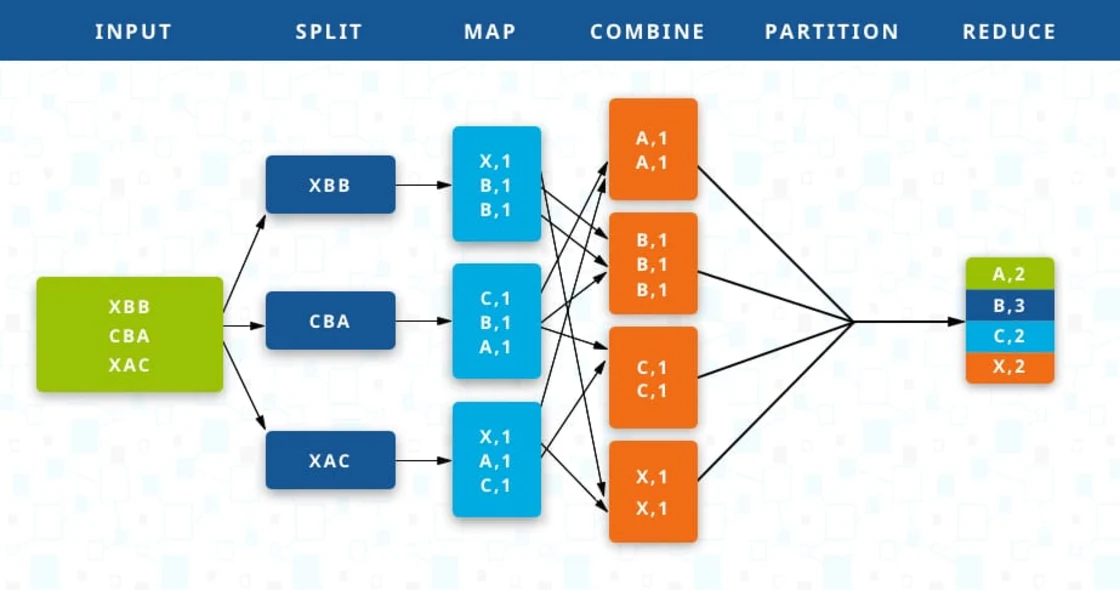
\includegraphics[scale=0.4]{mapreduce.jpg}
    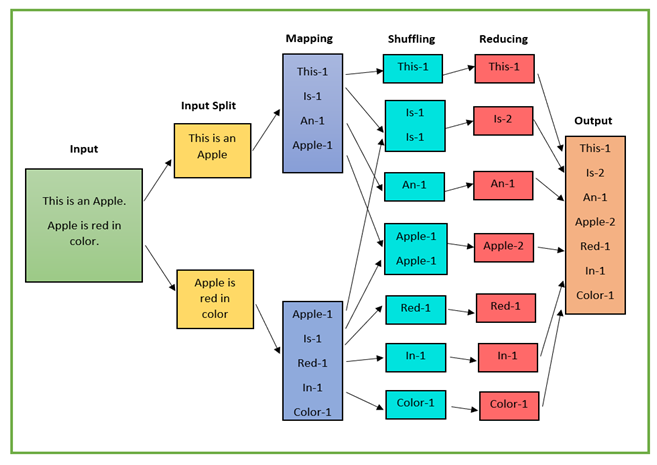
\includegraphics[scale=0.9]{map-reduce.png}
    \caption{https://www.analyticsvidhya.com/blog/2022/05/an-introduction-to-mapreduce-with-a-word-count-example/}
\end{figure}
\\
\\
De Data die verwerkt moet worden, doorloopt de volgende fases die telkens in parallel worden uitgevoerd:
\begin{itemize}
    \item \textbf{Opsplitsing}: grote volumes data worden opgesplitst en verdeeld over de HDFS nodes
    \item \textbf{Map}: elk deeltje data wordt bewerkt met de map functie en omgezet in sleutel-waarde paren (key-value pairs)
    \item \textbf{Herschikken en Sorteren}: De data-paren worden hergroepeerd op basis van de sleutels
    \item \textbf{Reduce}: de reduce functie ontvangt 
\end{itemize}

Hadoop ondersteunt het gebruik van MapReduce programmas geschreven in programmeertalen zoals Java, Python, Ruby en C++.
\autocite{Taylor2023}
\newline
\newline
Hadoop wordt o.a. alleenstaand gebruikt tijdens de oefeningen Big Data Processing, daarvoor kunnen we bestaande Docker Compose files gebruiken die de verschillende services bevatten nodig om een Master of Slave te starten.
In de eenvoudigste vorm is er 1 docker compose file die alle services opstart om te kunnen werken met 1 master en 1 slave.
\newline
\newline
Elke service (namenode, datanode, resourcemanager) is een specifiek Docker image, ook beschikbaar op DockerHub. Er zijn voorbeelden te vinden van de Docker scripts die gebruikt werden om dit soort images te bouwen. Typisch is er een basis Hadoop images dat het volledige framework bevat, en worden daar aparte images vanaf geleid die telkens maar 1 specifiek process (namenode, datanode, ...) van Hadoop opstarten.
Door op die manier met aparte images te werken kan het beheer van de cluster buiten Hadoop worden gedaan, bijvoorbeeld in Kubernetes.
\newline
\newline
In de volgende sectie gaan we Apache Spark bekijken, welke functionaliteit dit toevoegt aan Hadoop en hoe we dit kunnen integreren.
\newline
\newline

\section{Spark}
Apache Spark is net als Hadoop een Open Source framework bedoelt voor het verwerken van grote datasets. Spark verdeelt ook de gegevens en de taken over verschillende nodes, maar houdt data daarbij zoveel mogelijk in het RAM geheugen, in plaats van in een bestandssysteem. Voor bepaalde gevallen zal het dus sneller zijn dan Hadoop maar gezien het gebruik van geheugen is het beperkter in volume van data.
\newline
\autocite{AwsAmazon2023a}
\newline
De data in Spark wordt verdeeld opgeslagen in de cluster, in eerdere versies in RDD (Resilient Distributed Dataset), een set van data objecten in Java of Scala formaat. In nieuwere versies van Spark wordt DataFrame gebruikt, waarbij de gegevens gestructureerd worden in kolommen, gelijkaardig aan een tabel in een relationele databank. Volgende componenten zijn aanwezig in Spark om dit soort gestructureerde data te helpen verwerken: Spark SQL, Spark MLlib en Spark GraphX.
\autocite{DataFlair2023}
\newline
\newline


\subsection{Spark SQL, DataFrames and Datasets}
Deze module is de meest gebruikte Spark module voor gestructureerde data verwerking en laat toe om data op te halen en te bewerken door middel van SQL APIs, DataFrame APIs en Dataset APIs, waarvoor bibliotheken beschikbaar zijn voor meerdere programmeertalen waaronder Java, Scala en Python. Voor deze laatste zijn geen Dataset APIs beschikbaar.
De API voelt vertrouwd aan en begint met het openen van een Spark sessie via dewelke de data dan kan opgehaald worden uit een hele resem ondersteunde data sources (json, csv, text, hive, avro). Het ophalen gebeurt door gebruik te maken van de APIs, aangevuld met SQL instructies voor filteren en sorteren, waarna de data als Dataframe dan verder kan verwerkt worden.
De SQL interface kan ook aangesproken worden via jdbc en odbc.

(\autocite{Spark2023}, \autocite{Naveen2023}, \autocite{Spark2023a})


\subsection{Spark MLlib}
De Machine Learning Library (MLlib) van Apache Spark is ontworpen voor eenvoud en schaalbaarheid  en bestaat uit leeralgoritmen en hulpprogramma's, waaronder classificatie, regressie, clustering, collaboratieve filtering en onderliggende optimalisatie. Spark MLLib ondersteunt het trainen van modellen en daarop gebaseerde data voorspellingen, en integreert naadloos met de andere Spark-componenten. Het is beschikbaar voor meerdere programmeertalen waaronder Java, Scala en Python.
Spark MLlib biedt zowel een Dataframe API als eerste keus als een RDD API die intussen lijkt uitgefaseerd te worden.

\autocite{Spark2023b}

\subsection{Spark GraphX}
Spark GraphX is de Spark API die toelaat om grafen op te bouwen, gebaseerd op achterliggende databronnen in Spark, en hierop dan parallelle verwerking en analyses te doen. 
Een graaf is een data structuur die bestaat uit een verzameling objecten, knopen, en hun onderliggende relaties, verbindingen.
Spark GraphX bevat een steeds groter wordende set van graaf bouwers en algorithmes om graaf verwerking te ondersteunen.
(\autocite{Dayananda2019}, \autocite{Wikipedia2023})
\newline
\newline
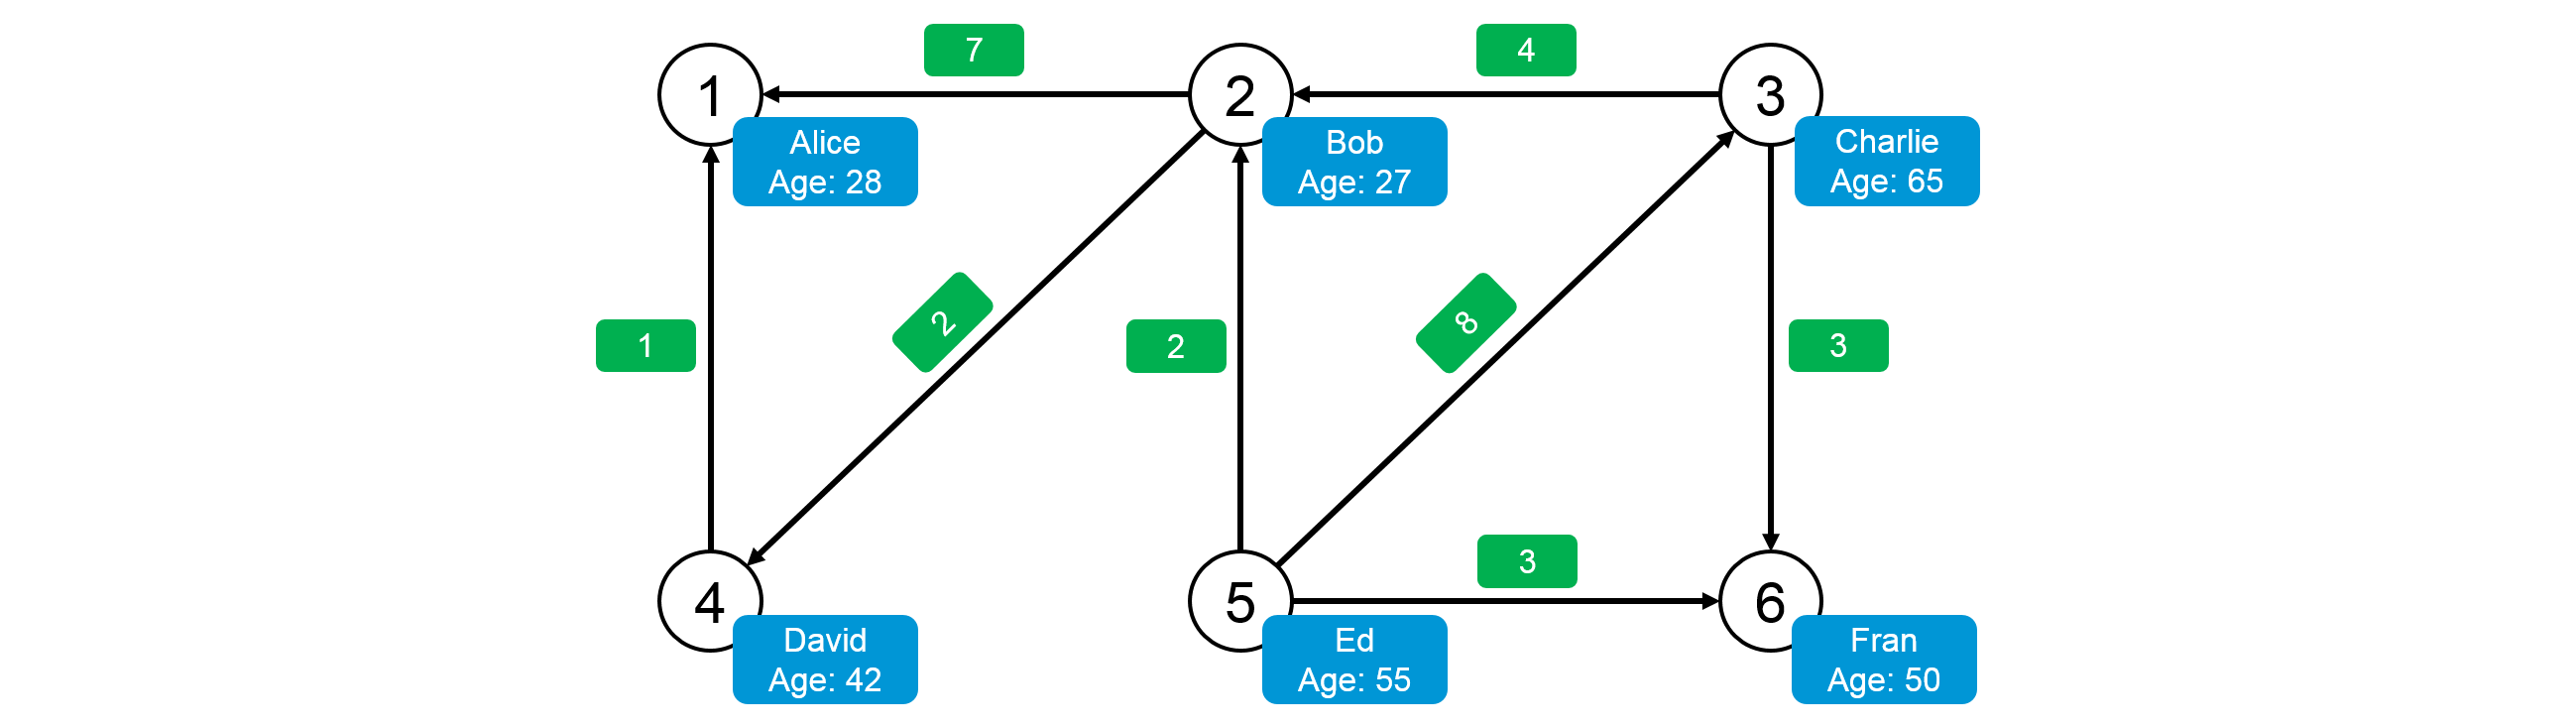
\includegraphics[scale=0.2]{GraphX-Example-Spark-GraphX-Tutorial-Edureka.png}
(https://www.edureka.co/blog/spark-graphx/)

\subsection{Spark Streaming / Structured Streaming}
Many applications need the ability to process and analyze not only batch data, but also streams of new data in real-time. Running on top of Spark, Spark Streaming enables powerful interactive and analytical applications across both streaming and historical data, while inheriting Spark’s ease of use and fault tolerance characteristics. It readily integrates with a wide variety of popular data sources, including HDFS, Flume, Kafka, and Twitter.\autocite{databricks2023}
\newline
\newline
Spark Streaming ondersteunt dus het verwerken van data in real-time met typische MapReduce algoritmes. Intussen wordt het als legacy beschouwd en is het vervangen door ``Structured Streaming'' dat gelijkaardige functionaliteit biedt door gebruik te maken van de DataFrame APIs in plaats van de Streaming RDD APIs. Met als voordeel dat SQL beter ondersteunt wordt in de DataFrame APIs.
\autocite{Buuck2022}
\newline
\newline
Het is dit laatste onderdeel, Spark Streaming, dat typisch in combinatie met Kafka (zie verder) wordt gebruikt om data van op te halen en na verwerking eventueel terug te bezorgen voor verdere stappen.
\newline
\newline
\newline
Terugkomend op ons doel van Spark in containers te draaien: er zijn Spark Docker images beschikbaar die toelaten zowel een Spark Master als een Spark Worker te starten.


\section{Kafka}
Apache Kafka is a distributed data store optimized for ingesting and processing streaming data in real-time. Streaming data is data that is continuously generated by thousands of data sources, which typically send the data records in simultaneously. A streaming platform needs to handle this constant influx of data, and process the data sequentially and incrementally.
\autocite{AwsAmazon2023b}

Apache Kafka is een Open Source gedistribueerd platform voor Event Streaming, waarbij binnenkomende boodschappen (events) continue worden opgeslagen en verwerkt, dat wordt gebruikt voor data-pijplijnen en data-integratie applicaties. Het is schaalbaar tot duizenden Brokers, kan billioenen boodschappen per dag aan en is zeer fault-tolerant door de cluster-architectuur. Hieronder worden een aantal typische concepten van Apache Kafka besproken.
\autocite{ASF2022b}

\subsection{Kafka Broker}
Een Kafka cluster bestaat uit meerdere servers, en deze servers worden Brokers genoemd. Brokers binnen een cluster praten rechtstreeks met elkaar of via Zookeeper (zie verder).
De belangrijkste taak van een Broker is het ontvangen en opslaan van Records.\autocite{GitBook2023}

\subsection{Event of Kafka record}
Een event is een boodschap die doorgeeft dat er ``iets'' is gebeurd, van belang voor de applicatie die wordt gebouwd. Deze boodschap bevat informatie over datgene dat is gebeurd en bevat een tijdstip, een sleutel, specifieke waardes en eventuele bijkomende metadata. Een voorbeeld uit de bankwereld van zo'n event is ``Piet Peeters'' ``heeft een betaling van 123Euro gedaan aan Jan Janssens'' op ``10/02/2023 om 11:35''.
In de terminologie van Kafka worden events gestuurd door ``Producers'' naar Kafka, waar ze worden verwerkt door ``Consumers''. Doordat beiden enkel via Kafka communiceren zijn ze van elkaar losgekoppeld en is dus de Producer niet afhankelijk van de beschikbaarheid van de Consumer, en kunnen eenvoudig meerdere Consumer bijgekoppeld worden zonder dat de Producer hiervan hoeft op de hoogte te zijn of worden aangepast. Dit wordt ook wel het ``Publish-Subscribe'' mechanisme genoemd. Er is 1 partij die events published en er zijn 1 of meerdere partijen die subscriben op de events van de Publisher.
In de terminologie van Kafka vormt een event een record dat opgeslagen wordt.
\autocite{Kafka2023}


\subsection{Kafka Topic}
Een Topic kan gezien worden als een soort logisch kanaal waarlangs de communicatie tussen Producer en Consumer verloopt. Een Producer stuurt dus Events naar een specifiek Topic en een Consumer gaat Events opvragen in datzelfde Topic. Het Topic is dus een begrip dat beiden kennen en een manier om ze aan elkaar te koppelen.
\autocite{Harbour2023}


\subsection{Kafka Partition}
Een Topic bestaat uit 1 of meerdere Partities. Records worden in een partitie opgeslagen, en door ze telkens achteraan de Partitie toe te voegen krijgen Consumers bij het lezen van een Topic/Partitie ze in dezelfde volgorde als ze gestuurd werden door de Consumer.
Meerdere partities voor 1 enkel Topic dienen ter ondersteuning van de schaalbaarheid, waarbij elke partitie wordt opgeslagen op een andere Broker. Op die manier kunnen Topics met zeer grote volumes aan records parallel opgeslagen en verwerkt worden.
\newline
\newline
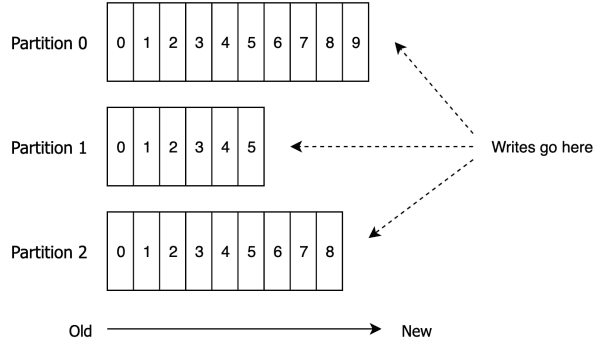
\includegraphics[scale=0.7]{Topic_with_partition.png}
\\
(https://codingharbour.com/apache-kafka/the-introduction-to-kafka-topics-and-partitions/)
\newline
\newline
Bij Partitions speelt de sleutel van een event een belangrijk aspect. Voor het verwerken van grote volumes aan events kunnen meerdere consumers opgezet worden die ieder de events van een enkele Partitie verwerken. Die Consumers krijgen de events van hun partitie in de juiste volgorde binnen, maar zien niet de events op de andere partities. Terugkerend naar ons voorbeeld uit de bankwereld:
\begin{itemize}
    \item Producer stuurt een event dat 100Euro op de rekening van Jan wordt gezet. Dit wordt op partitie 1 gezet.
    \item Producer stuurt een event dat 50Euro van de rekening van Jan wordt hgehaald. Dit wordt op partitie 2 gezet.
    \item Consumer X leest van de partitie 2 dat 50Euro van de rekening van Jan wordt hgehaald -> Dit wordt geweigerd want er staat niet genoeg geld op.
    \item Consumer Y leest van de partitie 1 dat 50Euro van de rekening van Jan wordt hgehaald -> Dit wordt uitgevoerd.
\end{itemize}

Om vorig scenario te vermijden worden events aan partities toegewezen op basis van de sleutel van het event. Het is dus aan de Producer om de juiste sleutel te kiezen, in dit geval ``Jan'', om ervoor te zorgen dat beide events op dezelfde partitie komen en allebei in de juiste volgorde aan de Consumer worden bezorgd..
\autocite{Harbour2023}
\newline
\newline


\section{Zookeeper}
ZooKeeper is een gedistribueerde service die het beheer van clusters en dus van grote hoeveelheden servers (nodes) helpt in goede banen te leiden. Dit op zich vormt een complexe taak en door die uit te besteden aan een oplossing zoals ZooKeeper kunnen andere gedistribueerde applicaties focusen op de eigen functionaliteiten en tijdens hun ontwikkeling geen tijd verliezen met het oplossen van de typische problemen zoals ``deadlock'', waarbij 2 processen op elkaar wachten en dus beide geblokkeerd zijn, en ``race conditions'' waarbij 2 processen een taak starten die slechts door 1 moet gedaan worden.  
Zookeeper houdt ook centraal bepaalde data bij, zoals configuratie informatie, en maakt die beschikbaar voor alle nodes.\autocite{ASF2023}
\newline
\newline 
Bij Apache Kafka werd Zookeeper gebruikt voor metadata beheer, bijvoorbeeld bijhouden welke brokers allemaal deelmaken van de cluster. Daarnaast helpt Zookeeper bij het kiezen van een broker die de leider moet worden van een bepaalde partitie. In recente versies is dit vervangen door een intern systeem, wat als voordeel heeft dat gebruikers dan geen extra applicatie moeten leren opzetten en er worden ook minder resources gebruikt.
\autocite{Conduktor2023}
\newline
\newline
Afhankelijk van de versie van Kafka die we uiteindelijk zullen gebruiken kan Zookeeper wel of niet toegevoegd worden aan de oplossing.
\newline
\newline

\section{Virtual IT Company (VIC)}
VIC is een ``bedrijf'' in HoGENT dat virtuele machines voorziet voor studenten, zodat bepaalde oplossingen niet op een eigen computer moeten draaien. Op aanvraag van studenten worden virtuele machine(s) opgezet en wordt er een soort van contract afgesproken met machine specs en lifespan.
\newline
\newline
De infrastructuur van VIC HoGent is gebaseerd op virtuele machines op de eigen hardware die wordt beheerd door VMware vSphere (VMware's virtualization platform) versie 8, waarvan de 2 belangrijkste onderdelen ESXi en vCenter Server zijn. ESXi is het virtualisatie platform waar virtuele machines worden uitgevoerd en vCenter Server is de service waarmee alles beheerd wordt.

\autocite{Saelens2023}

\subsection{Hypervisor}
Een hypervisor is software die op een fysieke machine draait en toelaat om op die machine meerdere virtual machines (VMs) te starten. Daartoe worden bepaalde resources van de fysieke machine, zoals geheugen, CPU en disk, gedeeld met alle virtuele machines.\autocite{VMware2023a}

\subsection{VMWare ESXi}
VMWare ESXi is de naam van de VMWare hypervisor.\autocite{VMware2023}

\subsection{vCenter Server}
vCenter Server is een tool van VMware die toelaat toe om centraal het beheer te doen van de ESXi hosts, de virtuele machines, de netwerkinfrastructuur, de opslag en de gerelateerde componenten.\autocite{Abbas2023}
\newline
\newline
De vSphere oplossing is leider in traditionele virtualisatie, gebaseerd op Virtuele machines. Applicatie virtualisatie, waarbij elke applicatie in een aparte container draait, wordt steeds belangrijker, en voor dit soort aanpak zijn Docker containers de standaard oplossing. Om hieraan tegemoet te komen werd door VMWare voor vSphere 6 'vSphere Integrated Containers' ontwikkeld, een oplossing die toelaat om Docker images en containers te gebruiken op bestaande vSphere infrastructuur. Toevallig noemt dit ook VIC.
Deze oplossing ondersteunt ook het deployen van Multi-Container Applicaties, o.a. door het gebruik van Docker Compose files.

\autocite{VMware2023b}


Intussen is Kubernetes de de-facto standaard geworden voor de orchestratie en het beheer van containers op grote schaal, dus zijn Docker containers en Kubernetes nu geïntegreerd vanaf vSphere versie 7. De 'vSphere Integrated Containers' oplossing van vSphere 6 wordt niet langer ondersteund en ook Docker Compose niet meer.

\autocite{VMware2021}


Kubernetes wordt door vSphere vooral ondersteund om Developers te laten werken met de door hun gekende tools, begrippen, Kubernetes configuratie files en processen zodat ze zich niet moeten verdiepen in VNWare vSphere. Ze hebben dan ook geen directe toegang of kennis nodig van de vSphere software.\autocite{VMware2019}

%\newline
%\newline
Daarnaast worden ook Docker containers ondersteund door VNWare vSphere, dus dit is een mogelijke oplossing zonder Kubernetes.
\newline
\newline
Kubernetes wordt door vSphere ondersteunt op 2 manieren: ofwel door gebruik te maken van de vSphere Pods waarbij het beheer van de Docker containers nog steeds via de traditionele vSphere Admin verloopt, die een subset van de Kubernetes configuratie ondersteunt, ofwel via de Tanzu Kubernetes cluster. Dit is software van VMWare die apart kan worden geïnstalleerd en die de Kubernetes manier van werken ondersteunt en dus ook meer controle biedt over het beheer van de Kubernetes cluster.
\newline
\newline
Zelf werken op de infrastructuur van VIC HoGent kan enkel onder supervisie en binnen beperkte tijden. Gezien de bachelorstage in combinatie met de bachelorproef was dit moeilijk en daarnaast was de beschikbaarheid van de co-promoter ook heel beperkt dus is er afgesproken dat de nodige informatie zou bezorgd worden die aantoont dat Kubernetes kan gebruikt worden op vSphere en zelf al het werk op een lokale Kubernetes installatie zou uitvoeren. Want momenteel wordt er nog geen Kubernetes gebruikt in het VIC. Ook geen Docker containers, alles is gebaseerd op virtuele machines. 
\newline
\newline
De volgende componenten zijn van belang om het gebruik van Kubernetes op VMware te begrijpen. De concepten van Kubernetes worden gelinkt aan VMWare concepten.
\newline
\newline
\subsection{Nodes}
Een Kubernetes node kan een virtuele of fysieke machine zijn die deel uitmaakt van een Kubernetes cluster en die centraal beheerd wordt.
Er zijn 2 types nodes:
\begin{itemize}
    \item ``master'' node: ook de ``control plane'' van Kubernetes genoemd. Deze controleert de volledige cluster en een cluster moet minstens 1 master node bevatten, en voor robustheid typisch 2.
    \item ``worker'' node: bevat de nodige services om Pods (zie verder) te kunnen starten, deze bevatten de containers.
\end{itemize}
\autocite{NirShtein2023}
%\newline
%\newline
\subsection{Pod}
Een Kubernetes Pod is een groep van 1 of meerdere containers die samen draaien in een gedeelde context. Een Pod wordt beheerd door de Kubelet software die op elke Node draait, de Kubelet zordt ervoor dat Pods herstart worden als ze onverwachts stoppen of als hun configuratie is gewijzigd. Die configuratie is gelijkaardig aan een Docker Compose files en bevat de 1 of meerdere container definities, de poorten die opengesteld moeten worden, de opslagvolumes, environment variabelen, enz.
\autocite{NirShtein2023}

Een master node komt overeen met vCenter Server en een worker node is een machine waarop de ESXi hypervisor draait, en die dus kan Pods starten. Vanuit VMware Administrator standpunt is een Pod gelijkaardig aan een virtuele machine.\autocite{VMware2019}



\subsection{Namespace}
Namespaces zijn een mechanisme om de beschikbare resources binnen een Kubernetes cluster in te delen in groepen en dan die groepen toe te wijzen aan teams van gebruikers of projecten. Dit is vooral nuttig indien meerdere personen rechtstreeks gebruik maken van Kubernetes om zelf containers te deployen. Dit is hier niet aan de orde dus Namespaces zijn van geen belang voor ons. Kubernets zelf stelt ook dat Namespaces niet bedoelf zijn voor clusters tot enkele tientallen gebruikers.
\autocite{Kubernetes2023c}

Namespaces zijn vergelijkbaar met vSphere Resource Pools.\autocite{VMware2019}
